\paragraph{La classe FilesManager}

\begin{minipage}
    {\linewidth}
    \centering
    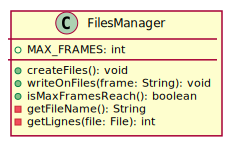
\includegraphics[width=0.80\linewidth]{../schemas/Conception_detaillee/classe_FilesManager.pdf}
    \captionof{figure}{Diagramme de classe de LogManager}
\end{minipage}

\subparagraph{Philosophie de conception \newline} 

\medspace

La classe FilesManager a pour rôle de créer et d'écrire sur un fichier sauvegardé sur le téléphone. 

\subparagraph{Description structurelle \newline}

\medspace

\textbf{Attributs :}

\begin{itemize}
    \item \textbf{MAX\_FRAMES: int} --- Nombre maximal de trames par fichier. 
\end{itemize}

\textbf{Services offerts :}

\begin{itemize}
    \item \textbf{createFiles() : void} --- Opération qui crée le fichier de sauvegarde des trames. 
    \item \textbf{writeOnFiles(frame : String ) : void } --- Opération qui écrit sur le fichier en cours la trame passée en paramètres. 
    \item \textbf{isMaxFramesReach() : bool } --- Opération qui vérifie si le nombre de trames est atteint dans le fichier. 
    \item \textbf{getFileName(): String} --- Opération qui permet de créer le nom du fichier de log.
    \item \textbf{getLignes(file: File): int} --- Opération qui permet de retourner le nombre de lignes présente dans le fichier. 
\end{itemize}